% =====================================================================
%  Основное содержимое отчёта (часть 1): структура, технологии,
%  алгоритмы, интерфейс.
% =====================================================================

\labpart{Структура разработанной системы}

Распознавание речи реализовано как новый сценарий использования поверх
архитектуры ЛР1--ЛР8 (см. \texttt{docs/ARCHITECTURE.md}). Тяжёлые
зависимости (модель Whisper, среда исполнения CTranslate2) изолированы
в том же \texttt{speech-service}, который появился в ЛР8 для синтеза
речи: оба направления -- «текст $\to$ речь» и «речь $\to$ текст» --
опираются на локальные нейросетевые модели и одинаковые ограничения по
ресурсам контейнера, поэтому отдельного микросервиса для распознавания
не потребовалось. Новыми стали эндпоинты и слой сопоставления фраз с
командами в \texttt{api}, таблица команд в БД и голосовой режим в
\texttt{frontend}. Структура системы на уровне контейнеров (C4,
уровень 2) показана на рисунке~\ref{fig:architecture-c4}; компоненты и
связи, добавленные в этой лабораторной работе, выделены зелёным цветом.

\pumldiagram{architecture-c4}{Диаграмма контейнеров разработанной системы (нотация C4); зелёным -- новое в ЛР9}{architecture-c4}{0.95}

Ответственность компонентов распределена следующим образом.
\begin{itemize}
  \item \textbf{\texttt{speech-service}} (Python, FastAPI,
  faster-whisper) -- эндпоинт \texttt{POST /stt} принимает аудиофайл
  (не более 25~МиБ), язык, подсказку-контекст (\texttt{initial\_prompt}),
  флаги фильтра тишины (\texttt{vad\_filter}) и выбора модели, а
  возвращает текст, определённый язык и время обработки. Используются
  две модели: \texttt{small} для распознавания записей целиком и более
  лёгкая \texttt{base} для потока, чтобы куски аудио не отставали от
  реального времени. Обе загружаются при старте контейнера в фоновом
  потоке, чтобы первое обращение пользователя не ждало загрузки
  модели;
  \item \textbf{\texttt{api}} (Python, FastAPI) -- \texttt{POST
  /speech/stt} (запись целиком), \texttt{WebSocket
  /speech/stt/stream} (поток: клиент присылает аудиокуски, сервер
  отвечает частичными результатами), CRUD-эндпоинты
  \texttt{/speech/commands} для списка команд и сопоставление
  распознанной фразы с командой. Число одновременных обращений к
  \texttt{speech-service} ограничено семафором (по умолчанию 4), чтобы
  несколько сеансов не превысили бюджет ядер контейнера; один кусок
  потока обрабатывается не более 20~с;
  \item \textbf{\texttt{postgres}} -- таблица \texttt{speech\_commands}
  (список операций, на которые реагирует система);
  \item \textbf{\texttt{frontend}} (React, TypeScript) -- захват
  микрофона, разбиение речи на фразы, отображение реакции и выполнение
  действия команды. Компоненты перечислены в
  таблице~\ref{tab:frontend-components}.
\end{itemize}

\begin{table}[H]
  \centering
  \caption{Компоненты интерфейса, реализующие распознавание речи}
  \label{tab:frontend-components}
  \small
  \begin{tabular}{|p{0.36\textwidth}|p{0.55\textwidth}|}
    \hline
    \textbf{Компонент} & \textbf{Назначение} \\
    \hline
    \texttt{useLiveSttStream} & Захват микрофона, запись кусками по 3{,}5~с, обмен с сервером по WebSocket, аварийное завершение сеанса \\
    \hline
    \texttt{SpeechModeContext}, \texttt{AssistantMicButton} & Голосовой режим: постоянное прослушивание команд из любого раздела приложения, кнопка-микрофон в правом нижнем углу, уведомления \\
    \hline
    \texttt{VoiceInputButton} & Микрофон в строке поиска и на вкладке «Распознавание речи» страницы «Настройки»: диктовка запроса с выполнением команд \\
    \hline
    \texttt{commandDispatch.ts}, \texttt{speechActions.ts} & Выполнение действия найденной команды; названия и подсказки действий \\
    \hline
    \texttt{matchCommand.ts} & Сопоставление фразы с командой на стороне браузера (зеркало серверной функции) \\
    \hline
    \texttt{micVolumeMeter.ts}, \texttt{liveSpeechRecognition.ts} & Уровень громкости микрофона (пульсация кнопки, обнаружение пауз); черновой субтитр Web Speech API \\
    \hline
    Вкладки «Распознавание речи» и «Команды» страницы «Настройки» & Выбор языка, фразы активации, проверка микрофона; добавление, изменение и удаление команд \\
    \hline
  \end{tabular}
\end{table}

\labpartbreak{Структура базы данных}

Для хранения списка операций добавлена одна таблица
\textbf{\texttt{speech\_commands}}, устроенная так (миграции \texttt{0016},
\texttt{0018} и \texttt{0023}):
\begin{itemize}
  \item \texttt{id} -- первичный ключ; порядок \texttt{id} определяет
  приоритет при сопоставлении (см. далее);
  \item \texttt{phrase} (до 200 символов) -- ключевая фраза, которую
  ищут в сказанном;
  \item \texttt{action} (до 50 символов) -- идентификатор действия из
  фиксированного набора (см. таблицу~\ref{tab:actions}): пользователь
  выбирает действие из списка, а не вводит произвольный код, поэтому
  добавить «несуществующую» команду нельзя;
  \item \texttt{language} (до 10 символов, по умолчанию \texttt{en}) --
  язык фразы: команда срабатывает только тогда, когда выбран тот же
  язык распознавания;
  \item \texttt{is\_active} -- флаг, позволяющий отключить команду,
  не удаляя её;
  \item \texttt{created\_at} -- время создания.
\end{itemize}

Миграции сразу заполняют таблицу начальным набором из 13 команд на
каждом из двух языков (английском и русском), покрывающим все
действия (см. таблицу~\ref{tab:actions}); этот набор пользователь
затем расширяет и меняет на вкладке «Команды» страницы «Настройки» без
переразвёртывания системы.

\labpartbreak{Задание списка операций}

Требование «задание списка операций, на которые система может
реагировать» реализовано как редактируемый список команд. Каждая
команда -- это пара «фраза $\to$ действие»; действий 13
(таблица~\ref{tab:actions}). Список доступен на вкладке «Команды»
страницы «Настройки»: команды добавляются, переименовываются,
переключаются между английским и русским языком, отключаются и
удаляются; после изменения список сразу перечитывается голосовым
режимом.

\begin{table}[H]
  \centering
  \caption{Действия системы и начальный набор фраз}
  \label{tab:actions}
  \small
  \begin{tabular}{|p{0.30\textwidth}|p{0.30\textwidth}|p{0.30\textwidth}|}
    \hline
    \textbf{Действие} & \textbf{Английская фраза} & \textbf{Русская фраза} \\
    \hline
    Перейти к поиску и выполнить запрос (сказанное как запрос) & search for \ldots & найди \ldots \\
    \hline
    Очистить поле запроса & clear search & очисти запрос \\
    \hline
    Озвучить открытый документ (или первый доступный на странице текст: реферат, перевод) & read this & прочитай это \\
    \hline
    Остановить озвучивание & stop reading & хватит читать \\
    \hline
    Открыть «Кроулинг» & go to crawling & перейди к краулингу \\
    \hline
    Открыть «Коллекции» & go to collections & перейди к коллекциям \\
    \hline
    Открыть «Поиск» без запроса & go to search & перейди к поиску \\
    \hline
    Открыть «Метрики» & go to metrics & перейди к метрикам \\
    \hline
    Открыть «Язык» & go to language identification & перейди к определению языка \\
    \hline
    Открыть «Реферирование» & go to summarization & перейди к реферированию \\
    \hline
    Открыть «Перевод» & go to translation & перейди к переводу \\
    \hline
    Открыть «Настройки» & go to settings & перейди к настройкам \\
    \hline
    Открыть «Справку» & go to help & перейди к справке \\
    \hline
  \end{tabular}
\end{table}

Дополнительно к списку команд в настройках задаётся необязательная
\emph{фраза активации}: если она непуста, система реагирует только на
фразы, в которых эта фраза есть, и отбрасывает всё, что было сказано до
неё (например, для фразы «computer» команда произносится как «computer,
go to metrics»). Это защищает от случайных срабатываний в шумном
помещении, когда голосовой режим слушает постоянно.

\labpartbreak{Технологии и методики}

\textbf{Выбор технологии распознавания.} Методичка предлагает Sphinx4,
Microsoft Speech API, Google Speech API, React-speech-recognition (Web
Speech API) и нейросетевые библиотеки. Web Speech API в Chrome отправляет
звук на серверы Google и работает только в некоторых браузерах;
Sphinx4 и другие классические акустические модели заметно уступают
нейросетевым по точности на произвольной лексике, а научные статьи по
computer science полны редких терминов; облачные API требуют ключей и
передачи речи третьей стороне. Поэтому выбрана нейросетевая модель
\textbf{Whisper} в реализации \textbf{faster-whisper} 1.2.1 (среда
CTranslate2, квантование INT8, работа на CPU), запускаемая локально в
контейнере. Web Speech API не отброшен полностью, а используется для
одной вспомогательной цели: показывать пользователю черновой субтитр
сказанного по словам прямо во время речи, пока серверная модель ещё
обрабатывает кусок. Текст законченной фразы берётся из субтитра, если
он доступен (браузеры Chrome и Edge), а иначе склеивается из
серверных результатов по кускам.

\textbf{Две модели.} Точность растёт с размером модели, но растёт и
время обработки. Для записей целиком, где пользователь готов подождать
доли секунды, используется \texttt{small}; для потока -- \texttt{base}, у
которой обработка куска идёт заметно быстрее (см. таблицу
сравнения моделей в разделе «Результаты тестирования»).

\textbf{Подсказка-контекст.} Каждый следующий кусок потока
распознаётся с параметром \texttt{initial\_prompt}, равным последним
200 символам уже распознанного текста: модель учитывает предыдущий
контекст, поэтому фраза, разорванная границей кусков, не теряет
согласования, а научная лексика распознаётся стабильнее.

\textbf{Фильтр тишины.} В потоке включён \texttt{vad\_filter} (детектор
речевой активности Silero, встроенный в faster-whisper): куски, в
которых никто не говорит, возвращают пустой результат, а не
«галлюцинации» Whisper на шуме, для которых модель склонна выдавать
случайные фразы.

\textbf{Выбор естественного языка.} Пользователь выбирает язык
распознавания на вкладке «Распознавание речи» (английский или
русский); выбор передаётся в Whisper как явная подсказка языка,
чтобы модель не тратила время и точность на его определение, и
одновременно определяет, какие команды считаются действующими. Для
варианта~1 основной язык -- английский; русский добавлен как второй
язык и потребовал только русской озвучки списка команд (см. таблицу
действий) -- благодаря тому, что модель Whisper многоязычная, а список
команд хранится в БД.

\labpartbreak{Основные алгоритмы}

\textbf{Общая схема потокового распознавания.} Последовательность
обмена сообщениями при потоковом распознавании показана на
рисунке~\ref{fig:stt-stream-sequence}. Браузер записывает звук
кусками по 3{,}5~с (запись останавливается и запускается заново, чтобы
каждый кусок был независимым и самодостаточным аудиофайлом, который
Whisper способен декодировать), отправляет их по WebSocket, а в ответ
получает текст каждого куска.

\pumldiagram{stt-stream-sequence}{Потоковое распознавание речи по WebSocket}{stt-stream-sequence}{0.95}

\textbf{Разбиение речи на фразы по паузам.} Автоматическая реакция
системы на речь требует решить, когда фраза закончилась. Разбиение на
равные интервалы времени (например, по 3{,}5~с) режет длинные фразы на
части, поэтому команда, попавшая на границу двух кусков, теряется.
Вместо этого система копит распознанный текст и оценивает
\emph{паузу по громкости микрофона}: уровень определяется как
среднеквадратичное значение сигнала (RMS), измеряемое через
\texttt{AnalyserNode} Web Audio API и масштабируемое коэффициентом 4 до
диапазона от 0 до 1. Пока уровень выше порога $0{,}06$, пользователь
считается говорящим. Накопленный текст считается законченной фразой,
когда после речи наступила тишина более 1{,}8~с (и субтитр Web Speech API
не менялся последние 0{,}5~с) либо фраза длится дольше 12~с
(рисунок~\ref{fig:utterance-segmentation}). Если браузер не позволяет
измерить громкость, каждый серверный кусок считается отдельной
фразой.

\pumldiagram{utterance-segmentation}{Непрерывное прослушивание: разбиение на фразы и реакция на команду}{utterance-segmentation}{1.0}

\textbf{Сопоставление фразы с командой.} Алгоритм
(рисунок~\ref{fig:command-matching}) намеренно прост и предсказуем:
текст и фраза команды нормализуются (знаки препинания заменяются
пробелами, регистр приводится к нижнему), после чего команда
считается сработавшей, если её фраза \emph{входит} в текст как
подстрока; из нескольких подходящих выбирается первая по порядку
\texttt{id}. Подстрока, а не точное совпадение, потому что Whisper
добавляет к фразе знаки препинания и слова-паразиты («Okay, go to
settings.»), а команда «search for \ldots» по определению содержит
произвольный хвост. Фразы начального набора подобраны так, чтобы ни одна
не была подстрокой другой (иначе более короткая перехватила бы более
длинную). Цена простоты -- ложные срабатывания на обычных предложениях,
содержащих фразу команды (см. «Результаты тестирования» и «Анализ
результатов»).

\pumldiagram{command-matching}{Сопоставление фразы с командой}{command-matching}{0.6}

Сопоставление выполняется и на сервере (для потока -- по сообщению
\texttt{stop}, для записи целиком -- в ответе \texttt{POST /speech/stt}),
и на клиенте (функция-зеркало \texttt{matchCommand.ts}): клиентское
сопоставление позволяет реагировать на каждую фразу, не дожидаясь
завершения всего сеанса, а серверное -- отвечает за режим «записал --
получил результат». Обе реализации отбирают только команды выбранного
языка распознавания.

\textbf{Действие и уведомление пользователя.} Когда команда найдена,
система (а) проигрывает по экрану зелёную волну от кнопки микрофона
(анимация длительностью 1{,}4~с), (б) выполняет действие
(\texttt{dispatchSpeechCommandAction}): переход на страницу,
подстановка запроса, очистка поля, озвучивание документа или
остановка озвучивания, (в) показывает уведомление с названием
сработавшей команды. Пока пользователь говорит, рядом с кнопкой
показывается распознанный текст, а сама кнопка пульсирует в такт
громкости голоса; после завершения фразы, не совпавшей ни с одной
командой, текст остаётся на экране ещё 1{,}8~с, чтобы пользователь
видел, что система его услышала, но команду не поняла.

\textbf{Устойчивость непрерывного сеанса.} Сеанс может идти
неограниченно долго, поэтому в нём предусмотрено несколько защит.
Единичный сбой обработки куска считается временным и молча
пропускается; только три сбоя подряд останавливают прослушивание с
сообщением об ошибке. Потеря микрофона (например, его отключили) и
обрыв соединения распознаются и сообщаются пользователю. Повторный
запуск не создаёт второго параллельного сеанса. Задержанные
остановки предыдущего сеанса отменяются при запуске нового, чтобы
таймер завершения старого сеанса не закрыл только что начавшийся.

\labpartbreak{Способы использования и пользовательский интерфейс}

Реализованы три способа управлять системой голосом:
\begin{itemize}
  \item \textbf{Голосовой режим} -- кнопка-микрофон в правом нижнем
  углу любой страницы. После включения система постоянно слушает и
  выполняет любую команду из списка; так можно, не касаясь мыши,
  перейти в нужный раздел, озвучить открытый документ или остановить
  озвучивание;
  \item \textbf{Микрофон в строке поиска} -- диктовка поискового запроса:
  сказанная фраза попадает в поле, а если она совпала с командой,
  выполняется команда (например, «clear search» очищает поле).
  Микрофон слушает непрерывно, пока пользователь не нажмёт на него
  ещё раз; каждая новая фраза заменяет предыдущую;
  \item \textbf{Проверка распознавания} на странице «Настройки» -- то же
  поведение без выполнения команд, для проверки микрофона и качества
  распознавания выбранного языка.
\end{itemize}


\begin{figure}[H]
  \centering
  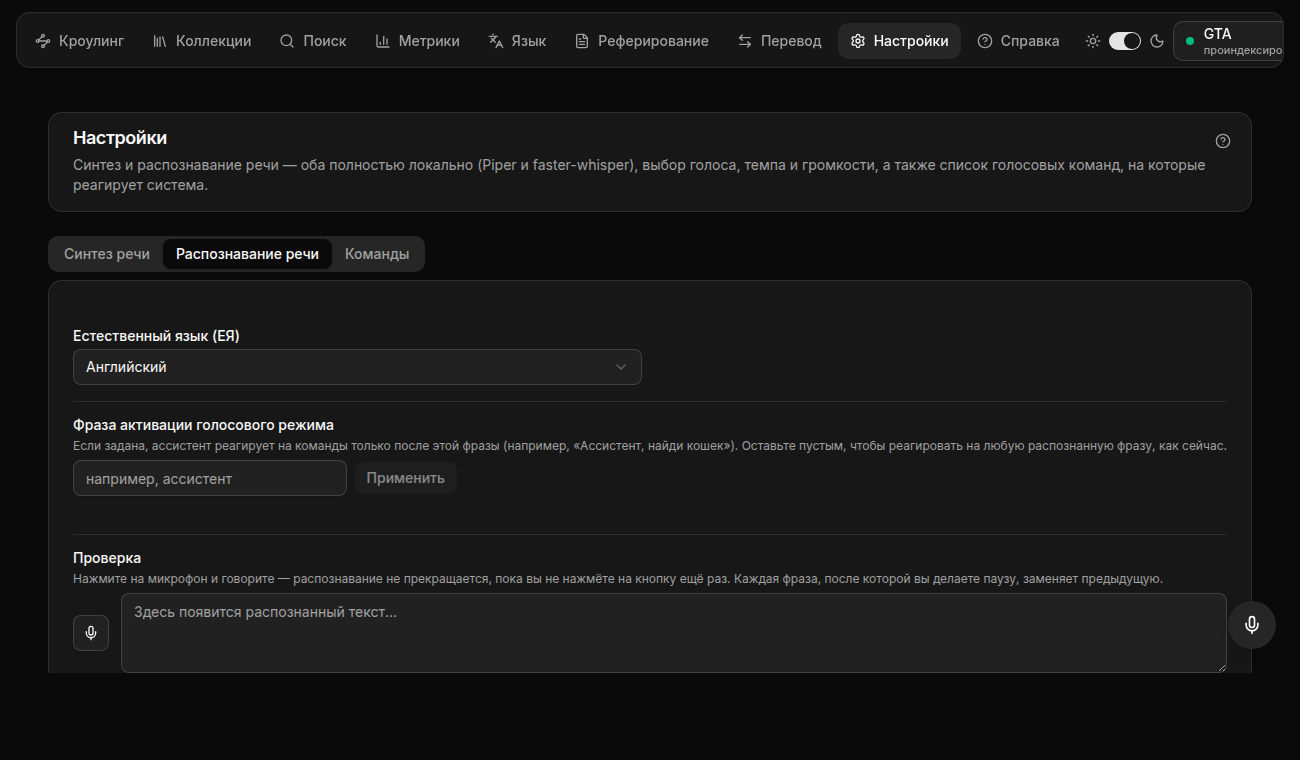
\includegraphics[width=\textwidth]{lab/pictures/settings_stt.png}
  \caption{Вкладка «Распознавание речи»: выбор языка, фраза активации, проверка микрофона}
  \label{fig:settings-stt}
\end{figure}

\begin{figure}[H]
  \centering
  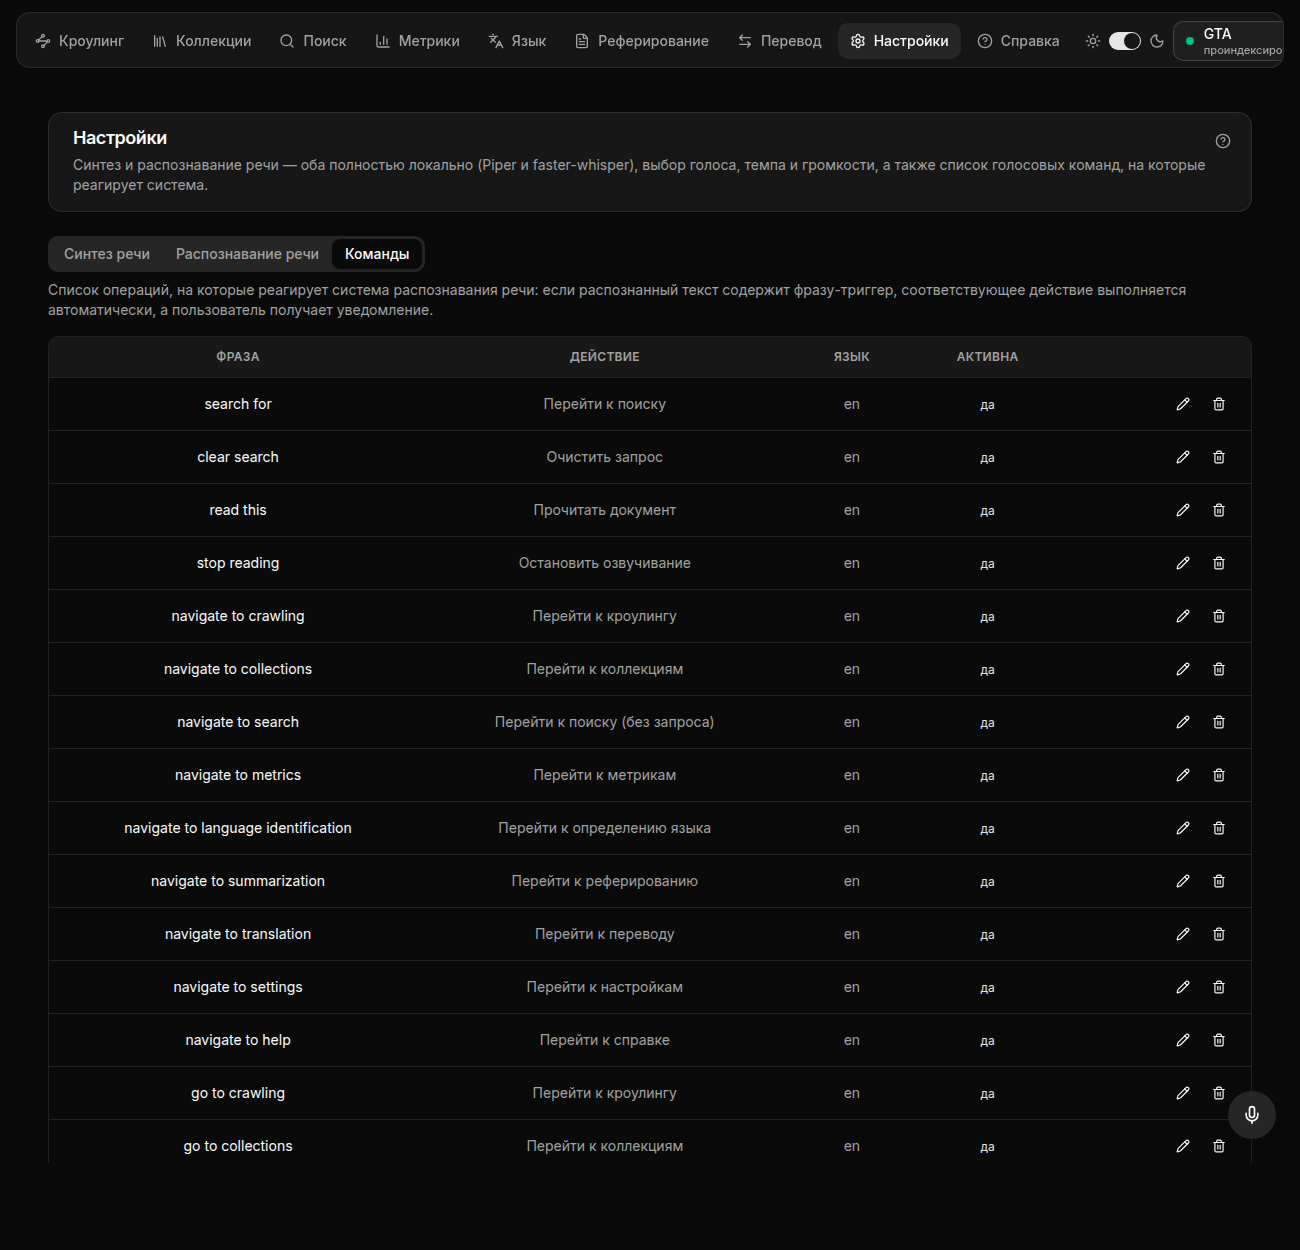
\includegraphics[width=\textwidth]{lab/pictures/settings_commands.png}
  \caption{Вкладка «Команды»: список операций, на которые реагирует система (добавление, изменение, отключение и удаление)}
  \label{fig:settings-commands}
\end{figure}

\begin{figure}[H]
  \centering
  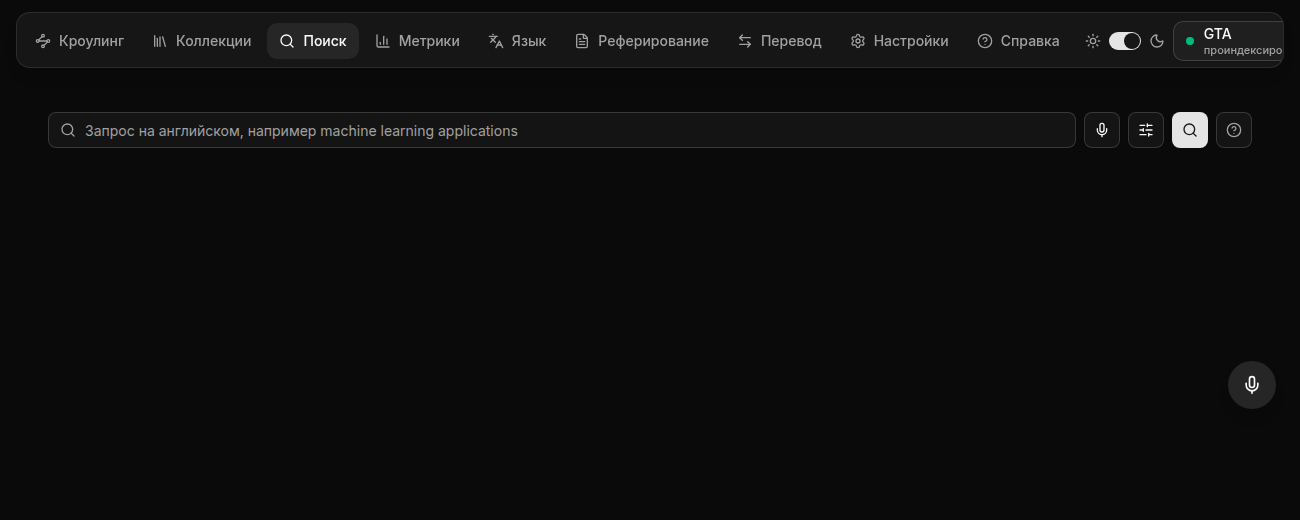
\includegraphics[width=\textwidth]{lab/pictures/search_mic.png}
  \caption{Страница «Поиск»: микрофон рядом со строкой запроса и кнопка голосового режима в правом нижнем углу}
  \label{fig:search-mic}
\end{figure}


\labpartbreak{Результаты тестирования}

\textbf{Методика.} Автоматическая проверка распознавания требует
записанной речи, а искать дикторов для сотен реплик невозможно,
поэтому тестовая речь \emph{синтезирована} голосами Piper из ЛР8 и
подана на вход \texttt{POST /speech/stt} (модель \texttt{small}) --
тот же эндпоинт, которым пользуется интерфейс, вместе с подстановкой
команд из БД. Английские реплики озвучены голосами Amy и Ryan (США) и
Alba (Великобритания), русские -- голосами Irina и Denis (Piper,
\texttt{ru\_RU}; в систему они не устанавливались, использовались только
для подготовки тестовых записей). Наборы:
\begin{itemize}
  \item \emph{команды} -- 13 английских и 13 русских фраз из
  таблицы~\ref{tab:actions}, каждая двумя голосами (по 26 записей);
  \item \emph{предложения} -- 10 английских предложений из области
  варианта (научные статьи по computer science) тремя голосами (30
  записей) и 5 русских двумя голосами (10 записей);
  \item \emph{не команды} -- обычные предложения, которые не должны
  вызывать никакого действия (7 английских, включая два трудных
  случая, и 5 русских, каждое двумя голосами).
\end{itemize}
Метрики: доля правильно найденных команд (найденная команда совпала с
ожидаемой), доля ошибочных слов WER (расстояние Левенштейна на уровне
слов между исходной фразой и распознанным текстом, нормализованное по
регистру и знакам препинания, на общем числе слов эталона), число
ложных срабатываний, время обработки. Контейнер был ограничен четырьмя
ядрами CPU.

\textbf{Ограничение методики.} Синтезированная речь чище живой: у неё
нет акцента, оговорок, дыхания и фонового шума микрофона. Поэтому
полученные ниже оценки надо рассматривать как \emph{верхнюю границу}
качества на реальной речи, а не как её прогноз; измерение на
записанной речи -- первое из предложений по улучшению. Русские
записи озвучены голосами Piper, которые сами по себе менее
естественны английских, так что часть русских ошибок может
объясняться не распознаванием, а качеством тестовой речи.

\textbf{Итоги по наборам} приведены в таблице~\ref{tab:stt-summary}.

\begin{table}[htbp]
  \centering
  \caption{Результаты распознавания синтезированной речи (модель \texttt{small})}
  \label{tab:stt-summary}
  \small
  \begin{tabular}{|>{\raggedright\arraybackslash}p{0.36\textwidth}|>{\raggedright\arraybackslash}p{0.12\textwidth}|>{\raggedright\arraybackslash}p{0.42\textwidth}|}
    \hline
    Набор & Записей & Результат \\
    \hline
    Английские команды & 26 & найдено верно 24 (92{,}3\,\%); Amy 13/13, Ryan 11/13; WER 3{,}8\,\% \\
    \hline
    Английские предложения (computer science) & 30 & WER 2{,}6\,\% (Amy 2{,}0, Ryan 2{,}0, Alba 3{,}9); без ошибок 24 из 30 \\
    \hline
    Английские не команды & 10 & ложных срабатываний 0 \\
    \hline
    Английские «трудные» предложения (содержат фразу команды) & 4 & ложных срабатываний 2 (оба раза -- «The search for optimal hyperparameters\ldots») \\
    \hline
    Русские команды & 26 & найдено верно 16 (61{,}5\,\%); Irina 10/13, Denis 6/13 \\
    \hline
    Русские предложения & 10 & WER 27{,}1\,\% (Irina 22{,}9, Denis 31{,}4) \\
    \hline
    Русские не команды & 10 & ложных срабатываний 0 \\
    \hline
  \end{tabular}
\end{table}

\textbf{Английский язык (основной по варианту).} Из 26 команд не
найдены две, и обе -- из-за ошибки распознавания, а не сопоставления:
«clear search» распознано как «CLEAR CERT», «go to settings» --
как «Build the settings.». Остальные фразы распознаны дословно, в том
числе «search for machine learning applications» с произвольным
хвостом. Предложения из предметной области распознаются с WER 2{,}6\,\%:
все ошибки -- на редких терминах («lemmatization» $\to$
«limitization», «hyperplane» $\to$ «hyperblane») и на артикле в
начале фразы. Единственные ложные срабатывания -- предложение
«The search for optimal hyperparameters is expensive»: оно содержит
фразу «search for», а алгоритм сопоставления по подстроке не
различает команду и обычное предложение с теми же словами. Второе
трудное предложение («Please go to the next section\ldots») не
вызвало срабатывания, так как ни одна команда не состоит из слов
«go to» без продолжения.

\textbf{Русский язык (дополнительный).} Распознавание заметно хуже:
верно найдено 16 команд из 26 (61{,}5\,\%), WER предложений -- 27{,}1\,\%.
Разрыв объясняется двумя причинами. Во-первых, русская морфология: ошибка
в одной букве окончания («коллекции» вместо «коллекциям»,
«реферировании» вместо «реферированию») ломает точное
сопоставление подстроки, хотя смысл фразы понятен. Во-вторых, узкоспециальные
слова, которых нет в обычной речи, распознаются с ошибками
(«краулингу» $\to$ «Каулинбу», «термов» $\to$ «темы», «булев» $\to$
«були»). Голос Denis дал 6 из 13 против 10 из 13 у Irina, что указывает
на влияние качества тестовой речи. Ложных срабатываний на русских
не командах не было.

\textbf{Две модели распознавания.} Модель \texttt{base}, которой
распознаётся поток, сравнена с \texttt{small} на тех же английских
записях (таблица~\ref{tab:stt-models}). \texttt{base} втрое быстрее, но
почти вдвое чаще ошибается. Для команд разница особенно заметна:
время обработки короткой фразы (1{,}2~с речи) у \texttt{small} -- 2{,}7~с,
то есть дольше самой фразы, у \texttt{base} -- 0{,}8~с. Заметная часть времени
\texttt{small} не зависит от длины фразы: модель обрабатывает аудио
окнами по 30~с, поэтому короткая команда стоит почти столько же, сколько
предложение втрое длиннее (2{,}7 против 2{,}4~с).

\begin{table}[H]
  \centering
  \caption{Сравнение моделей распознавания на английских записях}
  \label{tab:stt-models}
  \small
  \begin{tabular}{|>{\raggedright\arraybackslash}p{0.27\textwidth}|>{\raggedright\arraybackslash}p{0.14\textwidth}|>{\raggedright\arraybackslash}p{0.14\textwidth}|>{\raggedright\arraybackslash}p{0.15\textwidth}|>{\raggedright\arraybackslash}p{0.15\textwidth}|}
    \hline
    Модель & WER предложений, \% & WER команд, \% & Время, команда, с & Время, предложение, с \\
    \hline
    \texttt{small} (записи целиком) & 2{,}6 & 3{,}8 & 2{,}74 & 2{,}42 \\
    \hline
    \texttt{base} (поток) & 4{,}9 & 7{,}7 & 0{,}84 & 0{,}92 \\
    \hline
  \end{tabular}
\end{table}

\textbf{Устойчивость к шуму.} К десяти английским предложениям (голос
Amy) добавлялся гауссов шум с заданным отношением сигнал/шум (SNR);
результат -- в таблице~\ref{tab:stt-noise}. До SNR 5~дБ включительно
WER не изменился по сравнению с чистой записью (2{,}0\,\%), при 0~дБ
(шум по мощности равен речи) вырос до 5{,}9\,\%. Такая устойчивость --
следствие того, что Whisper обучен на очень разнообразных
данных, однако равномерный гауссов шум легче реального (музыка,
чужая речь, эхо помещения), поэтому реальный запас качества меньше.

\begin{table}[H]
  \centering
  \caption{Влияние шума на точность распознавания (10 английских предложений, голос Amy, модель \texttt{small})}
  \label{tab:stt-noise}
  \small
  \begin{tabular}{|c|c|c|c|c|}
    \hline
    Без шума & SNR 20~дБ & SNR 10~дБ & SNR 5~дБ & SNR 0~дБ \\
    \hline
    2{,}0\,\% & 2{,}0\,\% & 2{,}0\,\% & 2{,}0\,\% & 5{,}9\,\% \\
    \hline
  \end{tabular}
\end{table}

\textbf{Время реакции.} Слагаемые задержки от конца фразы до
выполнения команды в голосовом режиме: пауза до признания фразы
законченной (1{,}8~с -- задаётся константой) плюс время обработки
последнего куска потока (около 0{,}8--0{,}9~с у модели \texttt{base}, см.
таблицу~\ref{tab:stt-models}); распознавание идёт по кускам параллельно
с речью, поэтому в реальности последний кусок обычно короче. То
есть команда выполняется приблизительно через 2{,}5--3~с после
окончания фразы; заметную долю задержки составляет именно
намеренная пауза, а не вычисления.

\textbf{Автоматические тесты.} Слой сопоставления фраз с
командами (\texttt{test\_speech\_domain.py}), сессия потока
(\texttt{test\_speech\_streaming\_domain.py}), службы распознавания и
списка команд с базой данных SQLite (\texttt{test\_speech\_application.py},
в том числе проверка того, что команды отбираются по выбранному языку) и
маршруты \texttt{speech-service} (\texttt{test\_routes.py}) покрыты
тестами; весь набор прошёл без ошибок (18 тестов \texttt{api} и 9
тестов \texttt{speech-service}). Тесты и измерения выше относятся к серверному распознаванию; в Chrome текст фразы может браться из черновика Web Speech API, качество которого здесь не измерялось. Поведение в браузере (микрофон,
пульсация, реакция на команду) автоматическими тестами не покрыто и
проверяется вручную.

\labpart{Анализ результатов и предложения по улучшению}

\textbf{Что показали измерения.}
\begin{enumerate}
  \item \emph{Для английского (вариант~1) качество достаточное.} На чистой
  речи 92\,\% команд находятся верно, а все ошибки распознавания
  приходятся на редкие слова. Дополнительные 8\,\% потерь -- это
  ошибки самой модели на коротких фразах без контекста: фраза из двух-трёх
  слов даёт Whisper мало информации.
  \item \emph{Русский язык поддержан, но слабее.} Причина -- не столько
  распознавание, сколько жёсткость сопоставления: команда не
  срабатывает при любом отличии окончания.
  \item \emph{Шум почти не влияет} (до 5~дБ), но это оценка по
  синтезированной речи и гауссову шуму.
  \item \emph{Задержка определяется паузой-порогом} (1{,}8~с) и
  скоростью модели: \texttt{small} обрабатывает даже короткую фразу
  дольше, чем она длится, поэтому для потока применяется \texttt{base}
  ценой почти двукратного роста ошибок.
  \item \emph{Сопоставление по подстроке приводит к ложным
  срабатываниям} на обычных предложениях, содержащих фразу команды
  («The search for\ldots»). В голосовом режиме, который слушает
  постоянно, такое предложение, сказанное вслух рядом с
  компьютером, перейдёт на страницу поиска.
\end{enumerate}

\textbf{Ограничения системы.}
\begin{itemize}
  \item Оценки получены на синтезированной, а не живой речи (см.
  «Ограничение методики»).
  \item Распознавание работает только в браузерах с MediaRecorder и
  WebSocket; чернового субтитра нет вне Chrome/Edge (Web Speech API), --
  но без него система работает, лишь без показа слов по ходу речи.
  \item Команда -- это фраза-подстрока: параметров в командах нет,
  кроме единственной «search for \ldots», где параметром служит
  весь текст.
  \item Русские команды заданы фиксированной формой окончаний.
  \item Распознавание идёт на CPU: на четырёх ядрах одновременно
  обслуживаются не более четырёх сеансов (семафор), остальные ждут.
\end{itemize}

\textbf{Предложения по улучшению.}
\begin{enumerate}
  \item \emph{Измерить качество на живой речи}: записать 50--100 реплик
  нескольких дикторов в реальных условиях (шум помещения, разные
  микрофоны) и повторить те же измерения.
  \item \emph{Нечёткое сопоставление команд}: сравнивать леммы слов
  (для русского -- через морфологический анализатор), либо допускать
  небольшое расстояние Левенштейна между словами фразы и распознанным
  текстом; это устранило бы часть русских промахов и ошибки вида
  «clear cert» $\to$ «clear search».
  \item \emph{Устранить ложные срабатывания}: требовать, чтобы фраза
  команды была в начале высказывания («search for X», но не
  «The search for X»), либо использовать фразу активации по
  умолчанию (сейчас она необязательна).
  \item \emph{Подсказка модели словарём команд}: передавать Whisper
  в \texttt{initial\_prompt} названия команд и специальные термины
  предметной области (краулинг, реферирование, TF-IDF), чтобы редкие слова
  распознавались увереннее.
  \item \emph{Ускорить распознавание команд}: для коротких фраз
  использовать модель \texttt{base} (с 3-кратным выигрышем во времени)
  при включённой проверке результата на совпадение с командой, а
  \texttt{small} оставить для диктовки.
  \item \emph{Определять язык автоматически} (Whisper это умеет) и
  выбирать список команд по результату, чтобы пользователю не
  требовалось переключать язык вручную.
  \item \emph{Голосовое подтверждение действия}: озвучивать
  сработавшую команду голосом Piper из ЛР8 («Открываю метрики»),
  замыкая цикл «речь $\to$ действие $\to$ речь».
\end{enumerate}
\labpartbreak{Использованные готовые компоненты}

\begin{table}[H]
  \centering
  \caption{Библиотеки, готовые данные и программные средства, использованные при реализации ЛР9 (дополнительно к перечисленным в отчётах по ЛР1--ЛР4 и ЛР8)}
  \label{tab:stack-stt}
  \small
  \begin{tabularx}{\textwidth}{|l|X|}
    \hline
    Компонент & Назначение \\
    \hline
    faster-whisper 1.2.1 (CTranslate2) & Реализация модели Whisper для
      распознавания речи на CPU с квантованием INT8; модели
      \texttt{small} (записи целиком) и \texttt{base} (поток),
      детектор речевой активности Silero VAD. \\
    \hline
    Whisper (OpenAI) & Многоязычная нейросетевая модель распознавания
      речи; используется как английский, так и русский язык. \\
    \hline
    FastAPI, WebSocket, httpx & Эндпоинты \texttt{POST /stt},
      \texttt{WebSocket /speech/stt/stream}, клиент проксирования
      (используются и в предыдущих лабораторных). \\
    \hline
    MediaRecorder, getUserMedia & Захват звука микрофона в браузере
      кусками (webm/opus). \\
    \hline
    Web Audio API (\texttt{AnalyserNode}) & Измерение уровня громкости
      микрофона: пульсация кнопки и определение пауз в речи. \\
    \hline
    Web Speech API (\texttt{SpeechRecognition}) & Только черновой
      субтитр во время речи; финальный текст фразы приходит с
      сервера. \\
    \hline
    SQLAlchemy, Alembic & Модель и миграции таблицы
      \texttt{speech\_commands} (уже использовались). \\
    \hline
    Piper (ЛР8) & Синтез тестовой речи для автоматизированной проверки
      распознавания (см. «Результаты тестирования»). \\
    \hline
  \end{tabularx}
\end{table}
